\documentclass[a4paper]{article}
\usepackage[]{graphicx}\usepackage[]{color}
% maxwidth is the original width if it is less than linewidth
% otherwise use linewidth (to make sure the graphics do not exceed the margin)
\makeatletter
\def\maxwidth{ %
  \ifdim\Gin@nat@width>\linewidth
    \linewidth
  \else
    \Gin@nat@width
  \fi
}
\makeatother

\definecolor{fgcolor}{rgb}{0.345, 0.345, 0.345}
\newcommand{\hlnum}[1]{\textcolor[rgb]{0.686,0.059,0.569}{#1}}%
\newcommand{\hlstr}[1]{\textcolor[rgb]{0.192,0.494,0.8}{#1}}%
\newcommand{\hlcom}[1]{\textcolor[rgb]{0.678,0.584,0.686}{\textit{#1}}}%
\newcommand{\hlopt}[1]{\textcolor[rgb]{0,0,0}{#1}}%
\newcommand{\hlstd}[1]{\textcolor[rgb]{0.345,0.345,0.345}{#1}}%
\newcommand{\hlkwa}[1]{\textcolor[rgb]{0.161,0.373,0.58}{\textbf{#1}}}%
\newcommand{\hlkwb}[1]{\textcolor[rgb]{0.69,0.353,0.396}{#1}}%
\newcommand{\hlkwc}[1]{\textcolor[rgb]{0.333,0.667,0.333}{#1}}%
\newcommand{\hlkwd}[1]{\textcolor[rgb]{0.737,0.353,0.396}{\textbf{#1}}}%
\let\hlipl\hlkwb

\usepackage{framed}
\makeatletter
\newenvironment{kframe}{%
 \def\at@end@of@kframe{}%
 \ifinner\ifhmode%
  \def\at@end@of@kframe{\end{minipage}}%
  \begin{minipage}{\columnwidth}%
 \fi\fi%
 \def\FrameCommand##1{\hskip\@totalleftmargin \hskip-\fboxsep
 \colorbox{shadecolor}{##1}\hskip-\fboxsep
     % There is no \\@totalrightmargin, so:
     \hskip-\linewidth \hskip-\@totalleftmargin \hskip\columnwidth}%
 \MakeFramed {\advance\hsize-\width
   \@totalleftmargin\z@ \linewidth\hsize
   \@setminipage}}%
 {\par\unskip\endMakeFramed%
 \at@end@of@kframe}
\makeatother

\definecolor{shadecolor}{rgb}{.97, .97, .97}
\definecolor{messagecolor}{rgb}{0, 0, 0}
\definecolor{warningcolor}{rgb}{1, 0, 1}
\definecolor{errorcolor}{rgb}{1, 0, 0}
\newenvironment{knitrout}{}{} % an empty environment to be redefined in TeX

\usepackage{alltt}
\newcommand{\SweaveOpts}[1]{}  % do not interfere with LaTeX
\newcommand{\SweaveInput}[1]{} % because they are not real TeX commands
\newcommand{\Sexpr}[1]{}       % will only be parsed by R




\usepackage[utf8]{inputenc}
%\usepackage[ngerman]{babel}
\usepackage{a4wide,paralist}
\usepackage{amsmath, amssymb, xfrac, amsthm}
\usepackage{dsfont}
\usepackage[usenames,dvipsnames]{xcolor}
\usepackage{amsfonts}
\usepackage{graphicx}
\usepackage{caption}
\usepackage{subcaption}
\usepackage{framed}
\usepackage{multirow}
\usepackage{bytefield}
\usepackage{csquotes}
\usepackage[breakable, theorems, skins]{tcolorbox}
\usepackage{hyperref}
\usepackage{cancel}
\usepackage{bm}


\input{../../style/common}

\tcbset{enhanced}

\DeclareRobustCommand{\mybox}[2][gray!20]{%
	\iffalse
	\begin{tcolorbox}[   %% Adjust the following parameters at will.
		breakable,
		left=0pt,
		right=0pt,
		top=0pt,
		bottom=0pt,
		colback=#1,
		colframe=#1,
		width=\dimexpr\linewidth\relax,
		enlarge left by=0mm,
		boxsep=5pt,
		arc=0pt,outer arc=0pt,
		]
		#2
	\end{tcolorbox}
	\fi
}

\DeclareRobustCommand{\myboxshow}[2][gray!20]{%
%	\iffalse
	\begin{tcolorbox}[   %% Adjust the following parameters at will.
		breakable,
		left=0pt,
		right=0pt,
		top=0pt,
		bottom=0pt,
		colback=#1,
		colframe=#1,
		width=\dimexpr\linewidth\relax,
		enlarge left by=0mm,
		boxsep=5pt,
		arc=0pt,outer arc=0pt,
		]
		#2
	\end{tcolorbox}
%	\fi
}


%exercise numbering
\renewcommand{\theenumi}{(\alph{enumi})}
\renewcommand{\theenumii}{\roman{enumii}}
\renewcommand\labelenumi{\theenumi}


\font \sfbold=cmssbx10

\setlength{\oddsidemargin}{0cm} \setlength{\textwidth}{16cm}


\sloppy
\parindent0em
\parskip0.5em
\topmargin-2.3 cm
\textheight25cm
\textwidth17.5cm
\oddsidemargin-0.8cm
\pagestyle{empty}

\newcommand{\kopf}[1] {
\hrule
\vspace{.15cm}
\begin{minipage}{\textwidth}
%akwardly i had to put \" here to make it compile correctly
	{\sf\bf Introduction to Machine Learning \hfill Exercise sheet #1\\
	 \url{https://introduction-to-machine-learning.netlify.app/} \hfill WiSe 2020/2021}
\end{minipage}
\vspace{.05cm}
\hrule
\vspace{1cm}}

\newenvironment{allgemein}
	{\noindent}{\vspace{1cm}}

\newcounter{aufg}
\newenvironment{aufgabe}
	{\refstepcounter{aufg}\textbf{Exercise \arabic{aufg}:}\\ \noindent}
	{\vspace{0.5cm}}

\newcounter{loes}
\newenvironment{loesung}
	{\refstepcounter{loes}\textbf{Solution \arabic{loes}:}\\\noindent}
	{\bigskip}
	
\newenvironment{bonusaufgabe}
	{\refstepcounter{aufg}\textbf{Exercise \arabic{aufg}*\footnote{This
	is a bonus exercise.}:}\\ \noindent}
	{\vspace{0.5cm}}

\newenvironment{bonusloesung}
	{\refstepcounter{loes}\textbf{Solution \arabic{loes}*:}\\\noindent}
	{\bigskip}



\begin{document}
% !Rnw weave = knitr



\input{../../latex-math/basic-math.tex}
\input{../../latex-math/basic-ml.tex}

\kopf{2}

\loesung{

\begin{enumerate}
\item[a)] $k = 3$
\begin{align*}
\hat{y} =& \frac{2 + 2 + 4}{3} = \frac{8}{3} \approx 2.67\\
\hat{y}_\mathrm{weighted} =& \frac{\frac{1}{2}\cdot 2 + \frac{1}{2}\cdot 2 + \frac{1}{2}\cdot 4}{\frac{3}{2}} = \frac{8}{3} \approx 2.67 \\
\end{align*}

\begin{knitrout}
\definecolor{shadecolor}{rgb}{0.969, 0.969, 0.969}\color{fgcolor}

{\centering 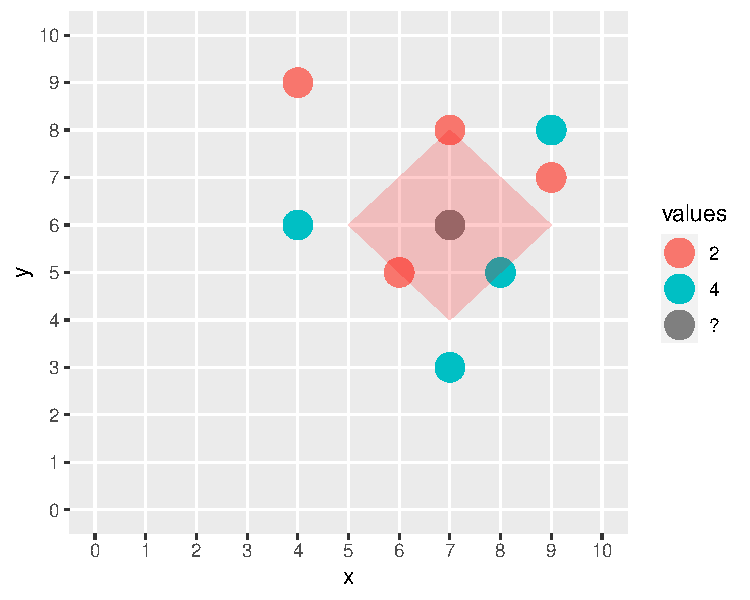
\includegraphics[width=\maxwidth]{figure/unnamed-chunk-3-1} 

}


\end{knitrout}

\item[b)] $k = 5$

\begin{align*}
\hat{y} =& \frac{2 + 2 + 2 + 4 + 4 + 4}{6} = 3 \\
\hat{y}_\mathrm{weighted} =& \frac{\frac{1}{2}\cdot 2 + \frac{1}{2}\cdot2 + \frac{1}{3} \cdot 2 +  \frac{1}{2}\cdot 4 + \frac{1}{3}\cdot 4 + \frac{1}{3}\cdot 4}{\frac{5}{2}} = \frac{44}{15} \approx 2.93\\
\end{align*}

\begin{knitrout}
\definecolor{shadecolor}{rgb}{0.969, 0.969, 0.969}\color{fgcolor}

{\centering 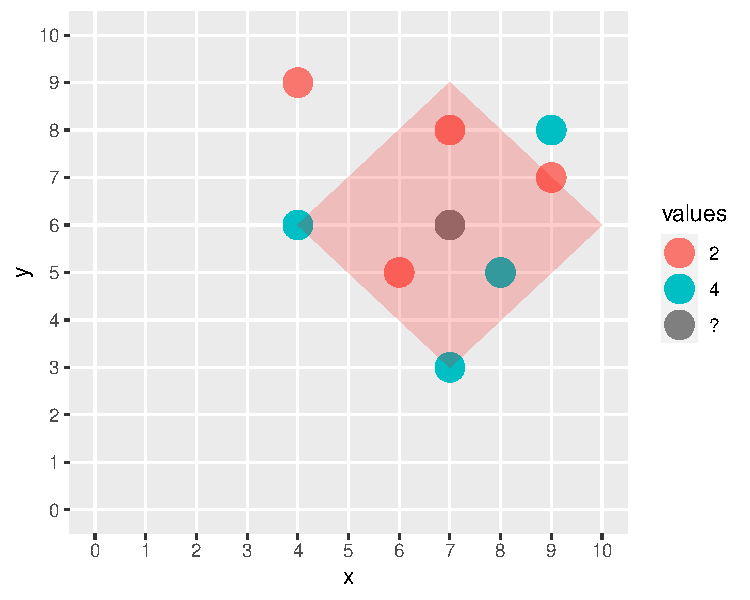
\includegraphics[width=\maxwidth]{figure/unnamed-chunk-4-1} 

}


\end{knitrout}

\item[c)] $k = 7$

\begin{align*}
\hat{y} =& \frac{2 + 2 + 2 + 4 + 4 + 4 + 4}{7} = \frac{22}{7} \approx 3.14\\
\hat{y}_\mathrm{weighted} =& \frac{\frac{1}{2}\cdot 2 + \frac{1}{2}\cdot2 + \frac{1}{3} \cdot 2 +  \frac{1}{2}\cdot 4 + \frac{1}{3}\cdot 4 + \frac{1}{3}\cdot 4 + \frac{1}{4} \cdot 4}{\frac{11}{4}} = \frac{100}{33} \approx 3.03\\
\end{align*}

\begin{knitrout}
\definecolor{shadecolor}{rgb}{0.969, 0.969, 0.969}\color{fgcolor}

{\centering 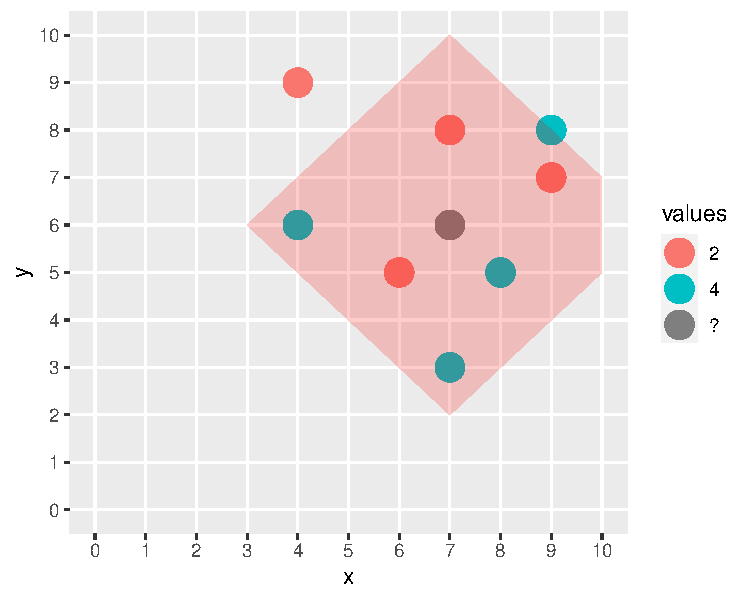
\includegraphics[width=\maxwidth]{figure/unnamed-chunk-5-1} 

}


\end{knitrout}

\end{enumerate}


  
}

\dlz

\loesung{

\begin{enumerate}
\item[a)] Learning consists of \textit{representation} (hypothesis space), 
\textit{evaluation} (risk) and \textit{optimization}. \\
A learner in mlr3 can be thought of as the implementation of these components, 
since 
\begin{itemize}
\item a representation of the associated model learnt from the data by 
using the implemented optimization is stored in such a learner object,
\item its performance measures can be accessed afterwards.
\end{itemize}
\item[b)] 
\begin{knitrout}
\definecolor{shadecolor}{rgb}{0.969, 0.969, 0.969}\color{fgcolor}\begin{kframe}
\begin{alltt}
\hlkwd{library}\hlstd{(mlr3)}
\hlkwd{library}\hlstd{(mlr3learners)}

\hlcom{# show all available learners}
\hlstd{mlr_learners}\hlopt{$}\hlkwd{keys}\hlstd{()}
\end{alltt}
\begin{verbatim}
##  [1] "classif.cv_glmnet"   "classif.debug"       "classif.featureless"
##  [4] "classif.glmnet"      "classif.kknn"        "classif.lda"        
##  [7] "classif.log_reg"     "classif.multinom"    "classif.naive_bayes"
## [10] "classif.nnet"        "classif.qda"         "classif.ranger"     
## [13] "classif.rpart"       "classif.svm"         "classif.xgboost"    
## [16] "regr.cv_glmnet"      "regr.featureless"    "regr.glmnet"        
## [19] "regr.kknn"           "regr.km"             "regr.lm"            
## [22] "regr.ranger"         "regr.rpart"          "regr.svm"           
## [25] "regr.xgboost"        "surv.cv_glmnet"      "surv.glmnet"        
## [28] "surv.ranger"         "surv.xgboost"
\end{verbatim}
\begin{alltt}
\hlcom{# see settings for a specific learner, e.g., for a regression tree}
\hlstd{rpart_learner} \hlkwb{<-} \hlkwd{lrn}\hlstd{(}\hlstr{"regr.rpart"}\hlstd{)}
\hlkwd{print}\hlstd{(rpart_learner)}
\end{alltt}
\begin{verbatim}
## <LearnerRegrRpart:regr.rpart>
## * Model: -
## * Parameters: xval=0
## * Packages: rpart
## * Predict Type: response
## * Feature types: logical, integer, numeric, factor, ordered
## * Properties: importance, missings, selected_features, weights
\end{verbatim}
\end{kframe}
\end{knitrout}


\end{enumerate}
}

\loesung{

See 
\href{https://github.com/compstat-lmu/lecture_i2ml/blob/master/exercises/supervised-regression/ex_rnw/sol_knn_lm.R}{R code}
}
\end{document}
